\documentclass[twoside]{book}

% Packages required by doxygen
\usepackage{fixltx2e}
\usepackage{calc}
\usepackage{doxygen}
\usepackage[export]{adjustbox} % also loads graphicx
\usepackage{graphicx}
\usepackage[utf8]{inputenc}
\usepackage{makeidx}
\usepackage{multicol}
\usepackage{multirow}
\PassOptionsToPackage{warn}{textcomp}
\usepackage{textcomp}
\usepackage[nointegrals]{wasysym}
\usepackage[table]{xcolor}

% Font selection
\usepackage[T1]{fontenc}
\usepackage[scaled=.90]{helvet}
\usepackage{courier}
\usepackage{amssymb}
\usepackage{sectsty}
\renewcommand{\familydefault}{\sfdefault}
\allsectionsfont{%
  \fontseries{bc}\selectfont%
  \color{darkgray}%
}
\renewcommand{\DoxyLabelFont}{%
  \fontseries{bc}\selectfont%
  \color{darkgray}%
}
\newcommand{\+}{\discretionary{\mbox{\scriptsize$\hookleftarrow$}}{}{}}

% Page & text layout
\usepackage{geometry}
\geometry{%
  a4paper,%
  top=2.5cm,%
  bottom=2.5cm,%
  left=2.5cm,%
  right=2.5cm%
}
\tolerance=750
\hfuzz=15pt
\hbadness=750
\setlength{\emergencystretch}{15pt}
\setlength{\parindent}{0cm}
\setlength{\parskip}{3ex plus 2ex minus 2ex}
\makeatletter
\renewcommand{\paragraph}{%
  \@startsection{paragraph}{4}{0ex}{-1.0ex}{1.0ex}{%
    \normalfont\normalsize\bfseries\SS@parafont%
  }%
}
\renewcommand{\subparagraph}{%
  \@startsection{subparagraph}{5}{0ex}{-1.0ex}{1.0ex}{%
    \normalfont\normalsize\bfseries\SS@subparafont%
  }%
}
\makeatother

% Headers & footers
\usepackage{fancyhdr}
\pagestyle{fancyplain}
\fancyhead[LE]{\fancyplain{}{\bfseries\thepage}}
\fancyhead[CE]{\fancyplain{}{}}
\fancyhead[RE]{\fancyplain{}{\bfseries\leftmark}}
\fancyhead[LO]{\fancyplain{}{\bfseries\rightmark}}
\fancyhead[CO]{\fancyplain{}{}}
\fancyhead[RO]{\fancyplain{}{\bfseries\thepage}}
\fancyfoot[LE]{\fancyplain{}{}}
\fancyfoot[CE]{\fancyplain{}{}}
\fancyfoot[RE]{\fancyplain{}{\bfseries\scriptsize Generated by Doxygen }}
\fancyfoot[LO]{\fancyplain{}{\bfseries\scriptsize Generated by Doxygen }}
\fancyfoot[CO]{\fancyplain{}{}}
\fancyfoot[RO]{\fancyplain{}{}}
\renewcommand{\footrulewidth}{0.4pt}
\renewcommand{\chaptermark}[1]{%
  \markboth{#1}{}%
}
\renewcommand{\sectionmark}[1]{%
  \markright{\thesection\ #1}%
}

% Indices & bibliography
\usepackage{natbib}
\usepackage[titles]{tocloft}
\setcounter{tocdepth}{3}
\setcounter{secnumdepth}{5}
\makeindex

% Hyperlinks (required, but should be loaded last)
\usepackage{ifpdf}
\ifpdf
  \usepackage[pdftex,pagebackref=true]{hyperref}
\else
  \usepackage[ps2pdf,pagebackref=true]{hyperref}
\fi
\hypersetup{%
  colorlinks=true,%
  linkcolor=blue,%
  citecolor=blue,%
  unicode%
}

% Custom commands
\newcommand{\clearemptydoublepage}{%
  \newpage{\pagestyle{empty}\cleardoublepage}%
}

\usepackage{caption}
\captionsetup{labelsep=space,justification=centering,font={bf},singlelinecheck=off,skip=4pt,position=top}

%===== C O N T E N T S =====

\begin{document}

% Titlepage & ToC
\hypersetup{pageanchor=false,
             bookmarksnumbered=true,
             pdfencoding=unicode
            }
\pagenumbering{alph}
\begin{titlepage}
\vspace*{7cm}
\begin{center}%
{\Large Weather\+Checking\+Rpi project }\\
\vspace*{1cm}
{\large Generated by Doxygen 1.8.13}\\
\end{center}
\end{titlepage}
\clearemptydoublepage
\pagenumbering{roman}
\tableofcontents
\clearemptydoublepage
\pagenumbering{arabic}
\hypersetup{pageanchor=true}

%--- Begin generated contents ---
\chapter{Brief Description}
\label{index}\hypertarget{index}{}\begin{DoxyAuthor}{Author}
Jérôme Lane, Katia Gasperi 
\end{DoxyAuthor}
\begin{DoxyDate}{Date}
30 April 2019 
\end{DoxyDate}
\begin{DoxyVersion}{Version}
1.\+1 
\end{DoxyVersion}
\hypertarget{index_intro_sec}{}\section{Introduction}\label{index_intro_sec}
Project where humidity, pressure and temperature are mesured with a Raspberry Pi 3 and B\+M\+E280 environmental sensor.~\newline
 Provide a graphical interface displaying these metrics.~\newline
 The interface provides a weather icon corresponding to the current weather trend.\hypertarget{index_requirements_sec}{}\section{Requirements}\label{index_requirements_sec}
\hypertarget{index_Hardware}{}\subsection{Hardware}\label{index_Hardware}

\begin{DoxyItemize}
\item Capteur B\+ME 280 
\item Raspberry PI 
\end{DoxyItemize}\hypertarget{index_Software}{}\subsection{Software}\label{index_Software}

\begin{DoxyItemize}
\item C/\+C++ 
\item Q\+ML 
\item Qt 
\end{DoxyItemize}\hypertarget{index_install_sec}{}\section{Installation}\label{index_install_sec}
Paquet debian \hypertarget{index_References}{}\section{References}\label{index_References}

\begin{DoxyItemize}
\item Algorithme de \hyperlink{class_zambretti}{Zambretti} 
\footnotesize \href{https://web.archive.org/web/20110610213848/http://www.meteormetrics.com/zambretti.htm}{\tt doc}
\normalsize 
\end{DoxyItemize}

~\newline
~\newline
 
\chapter{Hierarchical Index}
\section{Class Hierarchy}
This inheritance list is sorted roughly, but not completely, alphabetically\+:\begin{DoxyCompactList}
\item \contentsline{section}{App\+Model\+Private}{\pageref{class_app_model_private}}{}
\item Q\+Object\begin{DoxyCompactList}
\item \contentsline{section}{App\+Model}{\pageref{class_app_model}}{}
\item \contentsline{section}{Weather\+Data}{\pageref{class_weather_data}}{}
\end{DoxyCompactList}
\end{DoxyCompactList}

\chapter{Class Index}
\section{Class List}
Here are the classes, structs, unions and interfaces with brief descriptions\+:\begin{DoxyCompactList}
\item\contentsline{section}{\hyperlink{class_app_model}{App\+Model} }{\pageref{class_app_model}}{}
\item\contentsline{section}{\hyperlink{class_app_model_private}{App\+Model\+Private} }{\pageref{class_app_model_private}}{}
\item\contentsline{section}{\hyperlink{structbme280__calib__data}{bme280\+\_\+calib\+\_\+data} \\*Calibration data }{\pageref{structbme280__calib__data}}{}
\item\contentsline{section}{\hyperlink{structbme280__data}{bme280\+\_\+data} \\*Bme280 sensor structure which comprises of temperature, pressure and humidity data }{\pageref{structbme280__data}}{}
\item\contentsline{section}{\hyperlink{structbme280__dev}{bme280\+\_\+dev} \\*Bme280 device structure }{\pageref{structbme280__dev}}{}
\item\contentsline{section}{\hyperlink{structbme280__settings}{bme280\+\_\+settings} \\*Bme280 sensor settings structure which comprises of mode, oversampling and filter settings }{\pageref{structbme280__settings}}{}
\item\contentsline{section}{\hyperlink{structbme280__uncomp__data}{bme280\+\_\+uncomp\+\_\+data} \\*Bme280 sensor structure which comprises of uncompensated temperature, pressure and humidity data }{\pageref{structbme280__uncomp__data}}{}
\item\contentsline{section}{\hyperlink{structdata}{data} }{\pageref{structdata}}{}
\item\contentsline{section}{\hyperlink{structdatatab}{datatab} }{\pageref{structdatatab}}{}
\item\contentsline{section}{\hyperlink{class_db_manager}{Db\+Manager} }{\pageref{class_db_manager}}{}
\item\contentsline{section}{\hyperlink{class_db_table}{Db\+Table} }{\pageref{class_db_table}}{}
\item\contentsline{section}{\hyperlink{class_metrics_average}{Metrics\+Average} }{\pageref{class_metrics_average}}{}
\item\contentsline{section}{\hyperlink{class_weather_data}{Weather\+Data} }{\pageref{class_weather_data}}{}
\item\contentsline{section}{\hyperlink{class_zambretti}{Zambretti} }{\pageref{class_zambretti}}{}
\end{DoxyCompactList}

\chapter{File Index}
\section{File List}
Here is a list of all files with brief descriptions\+:\begin{DoxyCompactList}
\item\contentsline{section}{/home/jerome/projects/\+Weather\+Checking\+Rpi/weathercheckingrpi/\hyperlink{appmodel_8cpp}{appmodel.\+cpp} }{\pageref{appmodel_8cpp}}{}
\item\contentsline{section}{/home/jerome/projects/\+Weather\+Checking\+Rpi/weathercheckingrpi/\hyperlink{appmodel_8h}{appmodel.\+h} }{\pageref{appmodel_8h}}{}
\item\contentsline{section}{/home/jerome/projects/\+Weather\+Checking\+Rpi/weathercheckingrpi/\hyperlink{main_8cpp}{main.\+cpp} }{\pageref{main_8cpp}}{}
\end{DoxyCompactList}

\chapter{Class Documentation}
\hypertarget{class_app_model}{}\section{App\+Model Class Reference}
\label{class_app_model}\index{App\+Model@{App\+Model}}


\mbox{[}2\mbox{]}  




{\ttfamily \#include $<$appmodel.\+h$>$}



Inheritance diagram for App\+Model\+:\nopagebreak
\begin{figure}[H]
\begin{center}
\leavevmode
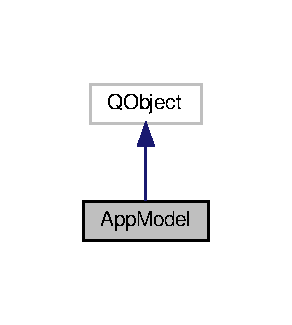
\includegraphics[width=140pt]{class_app_model__inherit__graph}
\end{center}
\end{figure}
\subsection*{Public Slots}
\begin{DoxyCompactItemize}
\item 
Q\+\_\+\+I\+N\+V\+O\+K\+A\+B\+LE void \hyperlink{class_app_model_a37e1da9d028779f7f0fc908e4c04fa76}{refresh\+Weather} ()
\begin{DoxyCompactList}\small\item\em \hyperlink{class_app_model_a37e1da9d028779f7f0fc908e4c04fa76}{App\+Model\+::refresh\+Weather} Access \href{http://api.openweathermap.org/data/2.5/weather}{\tt http\+://api.\+openweathermap.\+org/data/2.\+5/weather} site to get a specific city data Deals with connection errors. \end{DoxyCompactList}\end{DoxyCompactItemize}
\subsection*{Signals}
\begin{DoxyCompactItemize}
\item 
void \hyperlink{class_app_model_a574c2bd6f5c92ac9268107f8399989cb}{ready\+Changed} ()
\begin{DoxyCompactList}\small\item\em \mbox{[}3\mbox{]} \end{DoxyCompactList}\item 
void \hyperlink{class_app_model_af0007ee4da862433868baa5fdb31a3fe}{use\+Gps\+Changed} ()
\item 
void \hyperlink{class_app_model_a947db57e8c272bdb2420f3f273cd2e6a}{use\+Sensor\+Changed} ()
\item 
void \hyperlink{class_app_model_aeb28c7a57316aaf6295a943a65f60569}{city\+Changed} ()
\item 
void \hyperlink{class_app_model_a83e61455ed5672333b0db45f3f86417c}{weather\+Changed} ()
\end{DoxyCompactItemize}
\subsection*{Public Member Functions}
\begin{DoxyCompactItemize}
\item 
\hyperlink{class_app_model_affb3ea459bceb0650cdc810f3f5a2256}{App\+Model} (Q\+Object $\ast$parent=0)
\begin{DoxyCompactList}\small\item\em \mbox{[}0\mbox{]} \end{DoxyCompactList}\item 
\hyperlink{class_app_model_a67ab3004ccbe2822a8a0abb9fa96ace3}{$\sim$\+App\+Model} ()
\begin{DoxyCompactList}\small\item\em \mbox{[}1\mbox{]} \end{DoxyCompactList}\item 
bool \hyperlink{class_app_model_a3917fdc3dd8c97715991d9fd1a23abcc}{ready} () const
\item 
bool \hyperlink{class_app_model_a8ad68e982b0a307d9986ff538baedbd2}{has\+Source} () const
\item 
bool \hyperlink{class_app_model_a0e6e7506ba084133a6927d8c633ad699}{use\+Gps} () const
\item 
bool \hyperlink{class_app_model_a5b83f8c93976273d6e9f1664e62efe63}{use\+Sensor} () const
\item 
bool \hyperlink{class_app_model_aedeadab67d9bc5f5dfead369f66c3912}{has\+Valid\+City} () const
\item 
bool \hyperlink{class_app_model_a6ec5b34a1839a7141979709418174ad1}{has\+Valid\+Weather} () const
\item 
void \hyperlink{class_app_model_a81c3ffb3370837086366c9f70bb3d5eb}{set\+Use\+Gps} (bool value)
\item 
void \hyperlink{class_app_model_ac5fe590924b727724d9c686bb2552ed8}{had\+Error} (bool try\+Again)
\item 
void \hyperlink{class_app_model_ad1369130f74b4aabd0ac0d6b1b030014}{set\+Use\+Sensor} (bool value)
\item 
Q\+String \hyperlink{class_app_model_a093066c81b5fe2c1361df8fd19a21f51}{city} () const
\item 
void \hyperlink{class_app_model_ad0135d4a1551b6484ac28c434f861af5}{set\+City} (const Q\+String \&value)
\item 
\hyperlink{class_weather_data}{Weather\+Data} $\ast$ \hyperlink{class_app_model_a70a5bec8e359e4edbd16611efa96cf32}{weather} () const
\item 
Q\+Qml\+List\+Property$<$ \hyperlink{class_weather_data}{Weather\+Data} $>$ \hyperlink{class_app_model_aa9209b2390924841a009ab0d22b9a1b3}{forecast} () const
\end{DoxyCompactItemize}
\subsection*{Properties}
\begin{DoxyCompactItemize}
\item 
bool \hyperlink{class_app_model_a2af4f584bf701bff4546e889c16316d7}{ready}
\item 
bool \hyperlink{class_app_model_a2d25ce9151aea6a45cae797756a84445}{has\+Source}
\item 
bool \hyperlink{class_app_model_a98845ef5ffa3d9db0ee22aa3534b8608}{has\+Valid\+City}
\item 
bool \hyperlink{class_app_model_a493654987603c091935810e34e6b5c05}{has\+Valid\+Weather}
\item 
bool \hyperlink{class_app_model_aac827e2dce65eb299d4eec5ff4ab2155}{use\+Gps}
\item 
bool \hyperlink{class_app_model_ada296063fe2916580f532b639a546851}{use\+Sensor}
\item 
Q\+String \hyperlink{class_app_model_aa6915cabdaaf04805e00b5a2f75311e8}{city}
\item 
\hyperlink{class_weather_data}{Weather\+Data} \hyperlink{class_app_model_a72dfc16433c4ca50da689205e9db9298}{weather}
\item 
Q\+Qml\+List\+Property$<$ \hyperlink{class_weather_data}{Weather\+Data} $>$ \hyperlink{class_app_model_a3e45f56df91b1ad6d27c02c4ab1ad3c3}{forecast}
\end{DoxyCompactItemize}


\subsection{Detailed Description}
\mbox{[}2\mbox{]} 

\subsection{Constructor \& Destructor Documentation}
\mbox{\Hypertarget{class_app_model_affb3ea459bceb0650cdc810f3f5a2256}\label{class_app_model_affb3ea459bceb0650cdc810f3f5a2256}} 
\index{App\+Model@{App\+Model}!App\+Model@{App\+Model}}
\index{App\+Model@{App\+Model}!App\+Model@{App\+Model}}
\subsubsection{\texorpdfstring{App\+Model()}{AppModel()}}
{\footnotesize\ttfamily App\+Model\+::\+App\+Model (\begin{DoxyParamCaption}\item[{Q\+Object $\ast$}]{parent = {\ttfamily 0} }\end{DoxyParamCaption})\hspace{0.3cm}{\ttfamily [explicit]}}



\mbox{[}0\mbox{]} 

\mbox{[}0\mbox{]}

\mbox{[}1\mbox{]} \mbox{\Hypertarget{class_app_model_a67ab3004ccbe2822a8a0abb9fa96ace3}\label{class_app_model_a67ab3004ccbe2822a8a0abb9fa96ace3}} 
\index{App\+Model@{App\+Model}!````~App\+Model@{$\sim$\+App\+Model}}
\index{````~App\+Model@{$\sim$\+App\+Model}!App\+Model@{App\+Model}}
\subsubsection{\texorpdfstring{$\sim$\+App\+Model()}{~AppModel()}}
{\footnotesize\ttfamily App\+Model\+::$\sim$\+App\+Model (\begin{DoxyParamCaption}{ }\end{DoxyParamCaption})}



\mbox{[}1\mbox{]} 

Here is the call graph for this function\+:
\nopagebreak
\begin{figure}[H]
\begin{center}
\leavevmode
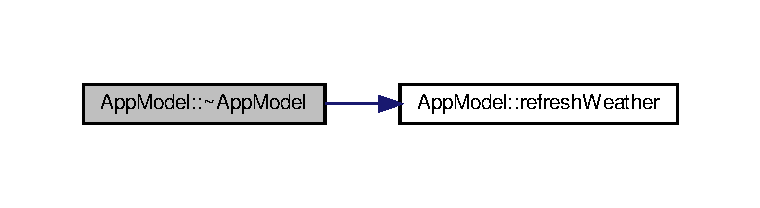
\includegraphics[width=350pt]{class_app_model_a67ab3004ccbe2822a8a0abb9fa96ace3_cgraph}
\end{center}
\end{figure}


\subsection{Member Function Documentation}
\mbox{\Hypertarget{class_app_model_a093066c81b5fe2c1361df8fd19a21f51}\label{class_app_model_a093066c81b5fe2c1361df8fd19a21f51}} 
\index{App\+Model@{App\+Model}!city@{city}}
\index{city@{city}!App\+Model@{App\+Model}}
\subsubsection{\texorpdfstring{city()}{city()}}
{\footnotesize\ttfamily Q\+String App\+Model\+::city (\begin{DoxyParamCaption}{ }\end{DoxyParamCaption}) const}

Here is the caller graph for this function\+:
\nopagebreak
\begin{figure}[H]
\begin{center}
\leavevmode
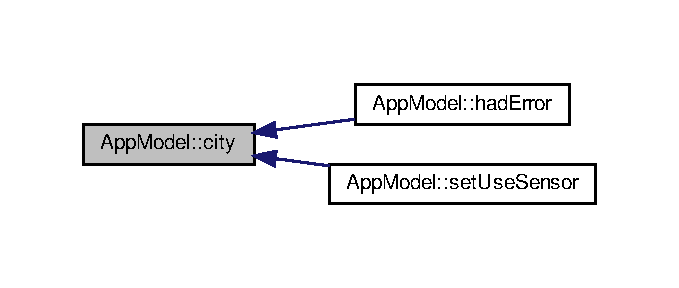
\includegraphics[width=326pt]{class_app_model_a093066c81b5fe2c1361df8fd19a21f51_icgraph}
\end{center}
\end{figure}
\mbox{\Hypertarget{class_app_model_aeb28c7a57316aaf6295a943a65f60569}\label{class_app_model_aeb28c7a57316aaf6295a943a65f60569}} 
\index{App\+Model@{App\+Model}!city\+Changed@{city\+Changed}}
\index{city\+Changed@{city\+Changed}!App\+Model@{App\+Model}}
\subsubsection{\texorpdfstring{city\+Changed}{cityChanged}}
{\footnotesize\ttfamily void App\+Model\+::city\+Changed (\begin{DoxyParamCaption}{ }\end{DoxyParamCaption})\hspace{0.3cm}{\ttfamily [signal]}}

Here is the caller graph for this function\+:
\nopagebreak
\begin{figure}[H]
\begin{center}
\leavevmode
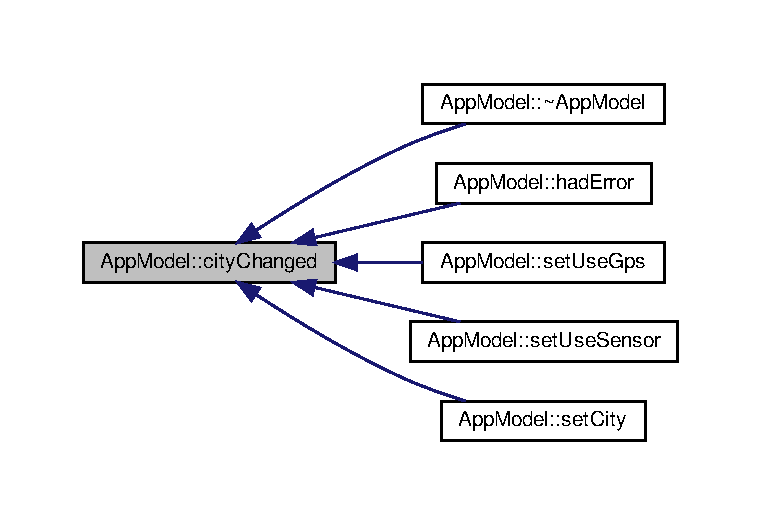
\includegraphics[width=350pt]{class_app_model_aeb28c7a57316aaf6295a943a65f60569_icgraph}
\end{center}
\end{figure}
\mbox{\Hypertarget{class_app_model_aa9209b2390924841a009ab0d22b9a1b3}\label{class_app_model_aa9209b2390924841a009ab0d22b9a1b3}} 
\index{App\+Model@{App\+Model}!forecast@{forecast}}
\index{forecast@{forecast}!App\+Model@{App\+Model}}
\subsubsection{\texorpdfstring{forecast()}{forecast()}}
{\footnotesize\ttfamily Q\+Qml\+List\+Property$<$\hyperlink{class_weather_data}{Weather\+Data}$>$ App\+Model\+::forecast (\begin{DoxyParamCaption}{ }\end{DoxyParamCaption}) const}

\mbox{\Hypertarget{class_app_model_ac5fe590924b727724d9c686bb2552ed8}\label{class_app_model_ac5fe590924b727724d9c686bb2552ed8}} 
\index{App\+Model@{App\+Model}!had\+Error@{had\+Error}}
\index{had\+Error@{had\+Error}!App\+Model@{App\+Model}}
\subsubsection{\texorpdfstring{had\+Error()}{hadError()}}
{\footnotesize\ttfamily void App\+Model\+::had\+Error (\begin{DoxyParamCaption}\item[{bool}]{try\+Again }\end{DoxyParamCaption})}

Manage time to wait before sending new request to get weather information before Here is the call graph for this function\+:
\nopagebreak
\begin{figure}[H]
\begin{center}
\leavevmode
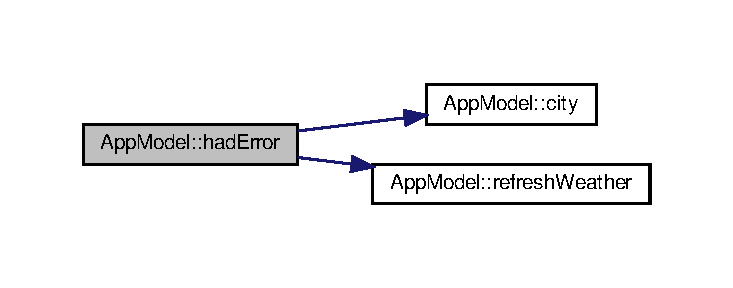
\includegraphics[width=350pt]{class_app_model_ac5fe590924b727724d9c686bb2552ed8_cgraph}
\end{center}
\end{figure}
\mbox{\Hypertarget{class_app_model_a8ad68e982b0a307d9986ff538baedbd2}\label{class_app_model_a8ad68e982b0a307d9986ff538baedbd2}} 
\index{App\+Model@{App\+Model}!has\+Source@{has\+Source}}
\index{has\+Source@{has\+Source}!App\+Model@{App\+Model}}
\subsubsection{\texorpdfstring{has\+Source()}{hasSource()}}
{\footnotesize\ttfamily bool App\+Model\+::has\+Source (\begin{DoxyParamCaption}{ }\end{DoxyParamCaption}) const}

\mbox{\Hypertarget{class_app_model_aedeadab67d9bc5f5dfead369f66c3912}\label{class_app_model_aedeadab67d9bc5f5dfead369f66c3912}} 
\index{App\+Model@{App\+Model}!has\+Valid\+City@{has\+Valid\+City}}
\index{has\+Valid\+City@{has\+Valid\+City}!App\+Model@{App\+Model}}
\subsubsection{\texorpdfstring{has\+Valid\+City()}{hasValidCity()}}
{\footnotesize\ttfamily bool App\+Model\+::has\+Valid\+City (\begin{DoxyParamCaption}{ }\end{DoxyParamCaption}) const}

\mbox{\Hypertarget{class_app_model_a6ec5b34a1839a7141979709418174ad1}\label{class_app_model_a6ec5b34a1839a7141979709418174ad1}} 
\index{App\+Model@{App\+Model}!has\+Valid\+Weather@{has\+Valid\+Weather}}
\index{has\+Valid\+Weather@{has\+Valid\+Weather}!App\+Model@{App\+Model}}
\subsubsection{\texorpdfstring{has\+Valid\+Weather()}{hasValidWeather()}}
{\footnotesize\ttfamily bool App\+Model\+::has\+Valid\+Weather (\begin{DoxyParamCaption}{ }\end{DoxyParamCaption}) const}

\mbox{\Hypertarget{class_app_model_a3917fdc3dd8c97715991d9fd1a23abcc}\label{class_app_model_a3917fdc3dd8c97715991d9fd1a23abcc}} 
\index{App\+Model@{App\+Model}!ready@{ready}}
\index{ready@{ready}!App\+Model@{App\+Model}}
\subsubsection{\texorpdfstring{ready()}{ready()}}
{\footnotesize\ttfamily bool App\+Model\+::ready (\begin{DoxyParamCaption}{ }\end{DoxyParamCaption}) const}

\mbox{\Hypertarget{class_app_model_a574c2bd6f5c92ac9268107f8399989cb}\label{class_app_model_a574c2bd6f5c92ac9268107f8399989cb}} 
\index{App\+Model@{App\+Model}!ready\+Changed@{ready\+Changed}}
\index{ready\+Changed@{ready\+Changed}!App\+Model@{App\+Model}}
\subsubsection{\texorpdfstring{ready\+Changed}{readyChanged}}
{\footnotesize\ttfamily void App\+Model\+::ready\+Changed (\begin{DoxyParamCaption}{ }\end{DoxyParamCaption})\hspace{0.3cm}{\ttfamily [signal]}}



\mbox{[}3\mbox{]} 

\mbox{\Hypertarget{class_app_model_a37e1da9d028779f7f0fc908e4c04fa76}\label{class_app_model_a37e1da9d028779f7f0fc908e4c04fa76}} 
\index{App\+Model@{App\+Model}!refresh\+Weather@{refresh\+Weather}}
\index{refresh\+Weather@{refresh\+Weather}!App\+Model@{App\+Model}}
\subsubsection{\texorpdfstring{refresh\+Weather}{refreshWeather}}
{\footnotesize\ttfamily void App\+Model\+::refresh\+Weather (\begin{DoxyParamCaption}{ }\end{DoxyParamCaption})\hspace{0.3cm}{\ttfamily [slot]}}



\hyperlink{class_app_model_a37e1da9d028779f7f0fc908e4c04fa76}{App\+Model\+::refresh\+Weather} Access \href{http://api.openweathermap.org/data/2.5/weather}{\tt http\+://api.\+openweathermap.\+org/data/2.\+5/weather} site to get a specific city data Deals with connection errors. 

Here is the caller graph for this function\+:
\nopagebreak
\begin{figure}[H]
\begin{center}
\leavevmode
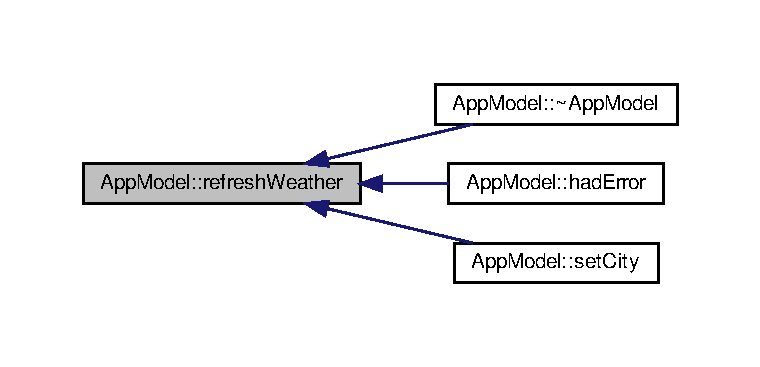
\includegraphics[width=350pt]{class_app_model_a37e1da9d028779f7f0fc908e4c04fa76_icgraph}
\end{center}
\end{figure}
\mbox{\Hypertarget{class_app_model_ad0135d4a1551b6484ac28c434f861af5}\label{class_app_model_ad0135d4a1551b6484ac28c434f861af5}} 
\index{App\+Model@{App\+Model}!set\+City@{set\+City}}
\index{set\+City@{set\+City}!App\+Model@{App\+Model}}
\subsubsection{\texorpdfstring{set\+City()}{setCity()}}
{\footnotesize\ttfamily void App\+Model\+::set\+City (\begin{DoxyParamCaption}\item[{const Q\+String \&}]{value }\end{DoxyParamCaption})}

Here is the call graph for this function\+:
\nopagebreak
\begin{figure}[H]
\begin{center}
\leavevmode
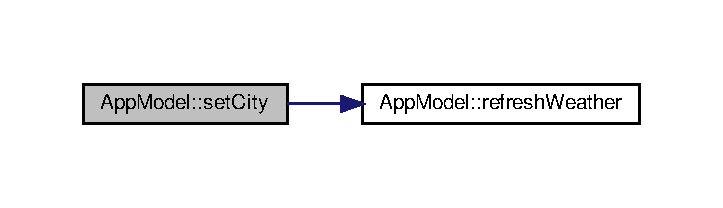
\includegraphics[width=347pt]{class_app_model_ad0135d4a1551b6484ac28c434f861af5_cgraph}
\end{center}
\end{figure}
\mbox{\Hypertarget{class_app_model_a81c3ffb3370837086366c9f70bb3d5eb}\label{class_app_model_a81c3ffb3370837086366c9f70bb3d5eb}} 
\index{App\+Model@{App\+Model}!set\+Use\+Gps@{set\+Use\+Gps}}
\index{set\+Use\+Gps@{set\+Use\+Gps}!App\+Model@{App\+Model}}
\subsubsection{\texorpdfstring{set\+Use\+Gps()}{setUseGps()}}
{\footnotesize\ttfamily void App\+Model\+::set\+Use\+Gps (\begin{DoxyParamCaption}\item[{bool}]{value }\end{DoxyParamCaption})}

Here is the call graph for this function\+:
\nopagebreak
\begin{figure}[H]
\begin{center}
\leavevmode
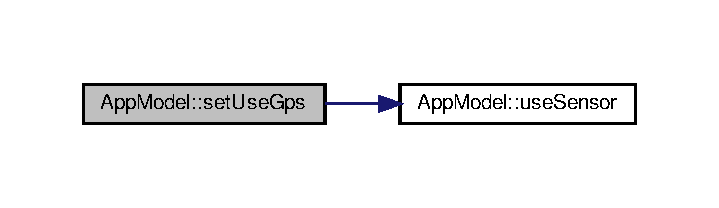
\includegraphics[width=345pt]{class_app_model_a81c3ffb3370837086366c9f70bb3d5eb_cgraph}
\end{center}
\end{figure}
\mbox{\Hypertarget{class_app_model_ad1369130f74b4aabd0ac0d6b1b030014}\label{class_app_model_ad1369130f74b4aabd0ac0d6b1b030014}} 
\index{App\+Model@{App\+Model}!set\+Use\+Sensor@{set\+Use\+Sensor}}
\index{set\+Use\+Sensor@{set\+Use\+Sensor}!App\+Model@{App\+Model}}
\subsubsection{\texorpdfstring{set\+Use\+Sensor()}{setUseSensor()}}
{\footnotesize\ttfamily void App\+Model\+::set\+Use\+Sensor (\begin{DoxyParamCaption}\item[{bool}]{value }\end{DoxyParamCaption})}

Here is the call graph for this function\+:
\nopagebreak
\begin{figure}[H]
\begin{center}
\leavevmode
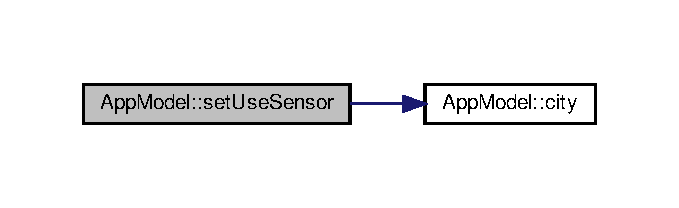
\includegraphics[width=326pt]{class_app_model_ad1369130f74b4aabd0ac0d6b1b030014_cgraph}
\end{center}
\end{figure}
\mbox{\Hypertarget{class_app_model_a0e6e7506ba084133a6927d8c633ad699}\label{class_app_model_a0e6e7506ba084133a6927d8c633ad699}} 
\index{App\+Model@{App\+Model}!use\+Gps@{use\+Gps}}
\index{use\+Gps@{use\+Gps}!App\+Model@{App\+Model}}
\subsubsection{\texorpdfstring{use\+Gps()}{useGps()}}
{\footnotesize\ttfamily bool App\+Model\+::use\+Gps (\begin{DoxyParamCaption}{ }\end{DoxyParamCaption}) const}

\mbox{\Hypertarget{class_app_model_af0007ee4da862433868baa5fdb31a3fe}\label{class_app_model_af0007ee4da862433868baa5fdb31a3fe}} 
\index{App\+Model@{App\+Model}!use\+Gps\+Changed@{use\+Gps\+Changed}}
\index{use\+Gps\+Changed@{use\+Gps\+Changed}!App\+Model@{App\+Model}}
\subsubsection{\texorpdfstring{use\+Gps\+Changed}{useGpsChanged}}
{\footnotesize\ttfamily void App\+Model\+::use\+Gps\+Changed (\begin{DoxyParamCaption}{ }\end{DoxyParamCaption})\hspace{0.3cm}{\ttfamily [signal]}}

Here is the caller graph for this function\+:
\nopagebreak
\begin{figure}[H]
\begin{center}
\leavevmode
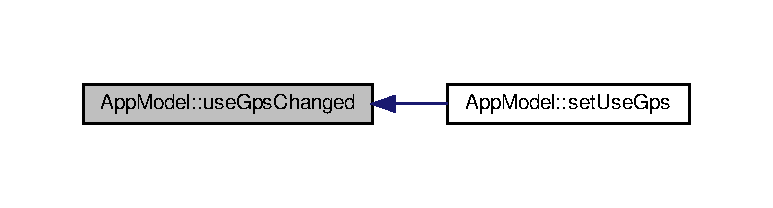
\includegraphics[width=350pt]{class_app_model_af0007ee4da862433868baa5fdb31a3fe_icgraph}
\end{center}
\end{figure}
\mbox{\Hypertarget{class_app_model_a5b83f8c93976273d6e9f1664e62efe63}\label{class_app_model_a5b83f8c93976273d6e9f1664e62efe63}} 
\index{App\+Model@{App\+Model}!use\+Sensor@{use\+Sensor}}
\index{use\+Sensor@{use\+Sensor}!App\+Model@{App\+Model}}
\subsubsection{\texorpdfstring{use\+Sensor()}{useSensor()}}
{\footnotesize\ttfamily bool App\+Model\+::use\+Sensor (\begin{DoxyParamCaption}{ }\end{DoxyParamCaption}) const}

Here is the caller graph for this function\+:
\nopagebreak
\begin{figure}[H]
\begin{center}
\leavevmode
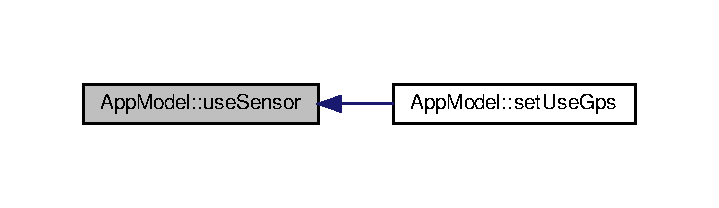
\includegraphics[width=345pt]{class_app_model_a5b83f8c93976273d6e9f1664e62efe63_icgraph}
\end{center}
\end{figure}
\mbox{\Hypertarget{class_app_model_a947db57e8c272bdb2420f3f273cd2e6a}\label{class_app_model_a947db57e8c272bdb2420f3f273cd2e6a}} 
\index{App\+Model@{App\+Model}!use\+Sensor\+Changed@{use\+Sensor\+Changed}}
\index{use\+Sensor\+Changed@{use\+Sensor\+Changed}!App\+Model@{App\+Model}}
\subsubsection{\texorpdfstring{use\+Sensor\+Changed}{useSensorChanged}}
{\footnotesize\ttfamily void App\+Model\+::use\+Sensor\+Changed (\begin{DoxyParamCaption}{ }\end{DoxyParamCaption})\hspace{0.3cm}{\ttfamily [signal]}}

Here is the caller graph for this function\+:
\nopagebreak
\begin{figure}[H]
\begin{center}
\leavevmode
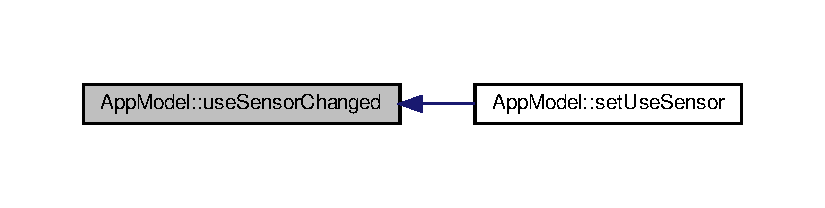
\includegraphics[width=350pt]{class_app_model_a947db57e8c272bdb2420f3f273cd2e6a_icgraph}
\end{center}
\end{figure}
\mbox{\Hypertarget{class_app_model_a70a5bec8e359e4edbd16611efa96cf32}\label{class_app_model_a70a5bec8e359e4edbd16611efa96cf32}} 
\index{App\+Model@{App\+Model}!weather@{weather}}
\index{weather@{weather}!App\+Model@{App\+Model}}
\subsubsection{\texorpdfstring{weather()}{weather()}}
{\footnotesize\ttfamily \hyperlink{class_weather_data}{Weather\+Data}$\ast$ App\+Model\+::weather (\begin{DoxyParamCaption}{ }\end{DoxyParamCaption}) const}

\mbox{\Hypertarget{class_app_model_a83e61455ed5672333b0db45f3f86417c}\label{class_app_model_a83e61455ed5672333b0db45f3f86417c}} 
\index{App\+Model@{App\+Model}!weather\+Changed@{weather\+Changed}}
\index{weather\+Changed@{weather\+Changed}!App\+Model@{App\+Model}}
\subsubsection{\texorpdfstring{weather\+Changed}{weatherChanged}}
{\footnotesize\ttfamily void App\+Model\+::weather\+Changed (\begin{DoxyParamCaption}{ }\end{DoxyParamCaption})\hspace{0.3cm}{\ttfamily [signal]}}

Here is the caller graph for this function\+:
\nopagebreak
\begin{figure}[H]
\begin{center}
\leavevmode
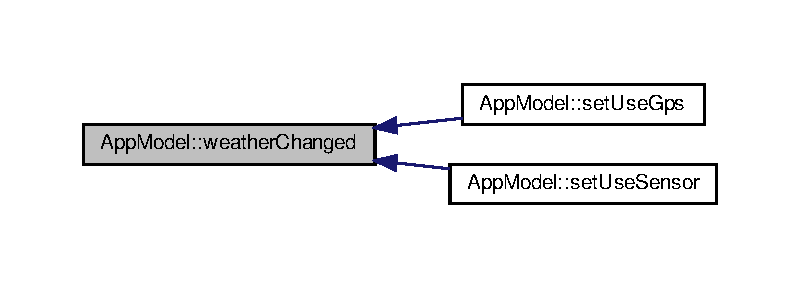
\includegraphics[width=350pt]{class_app_model_a83e61455ed5672333b0db45f3f86417c_icgraph}
\end{center}
\end{figure}


\subsection{Property Documentation}
\mbox{\Hypertarget{class_app_model_aa6915cabdaaf04805e00b5a2f75311e8}\label{class_app_model_aa6915cabdaaf04805e00b5a2f75311e8}} 
\index{App\+Model@{App\+Model}!city@{city}}
\index{city@{city}!App\+Model@{App\+Model}}
\subsubsection{\texorpdfstring{city}{city}}
{\footnotesize\ttfamily Q\+String App\+Model\+::city\hspace{0.3cm}{\ttfamily [read]}, {\ttfamily [write]}}

\mbox{\Hypertarget{class_app_model_a3e45f56df91b1ad6d27c02c4ab1ad3c3}\label{class_app_model_a3e45f56df91b1ad6d27c02c4ab1ad3c3}} 
\index{App\+Model@{App\+Model}!forecast@{forecast}}
\index{forecast@{forecast}!App\+Model@{App\+Model}}
\subsubsection{\texorpdfstring{forecast}{forecast}}
{\footnotesize\ttfamily Q\+Qml\+List\+Property$<$ \hyperlink{class_weather_data}{Weather\+Data} $>$ App\+Model\+::forecast\hspace{0.3cm}{\ttfamily [read]}}

\mbox{\Hypertarget{class_app_model_a2d25ce9151aea6a45cae797756a84445}\label{class_app_model_a2d25ce9151aea6a45cae797756a84445}} 
\index{App\+Model@{App\+Model}!has\+Source@{has\+Source}}
\index{has\+Source@{has\+Source}!App\+Model@{App\+Model}}
\subsubsection{\texorpdfstring{has\+Source}{hasSource}}
{\footnotesize\ttfamily bool App\+Model\+::has\+Source\hspace{0.3cm}{\ttfamily [read]}}

\mbox{\Hypertarget{class_app_model_a98845ef5ffa3d9db0ee22aa3534b8608}\label{class_app_model_a98845ef5ffa3d9db0ee22aa3534b8608}} 
\index{App\+Model@{App\+Model}!has\+Valid\+City@{has\+Valid\+City}}
\index{has\+Valid\+City@{has\+Valid\+City}!App\+Model@{App\+Model}}
\subsubsection{\texorpdfstring{has\+Valid\+City}{hasValidCity}}
{\footnotesize\ttfamily bool App\+Model\+::has\+Valid\+City\hspace{0.3cm}{\ttfamily [read]}}

\mbox{\Hypertarget{class_app_model_a493654987603c091935810e34e6b5c05}\label{class_app_model_a493654987603c091935810e34e6b5c05}} 
\index{App\+Model@{App\+Model}!has\+Valid\+Weather@{has\+Valid\+Weather}}
\index{has\+Valid\+Weather@{has\+Valid\+Weather}!App\+Model@{App\+Model}}
\subsubsection{\texorpdfstring{has\+Valid\+Weather}{hasValidWeather}}
{\footnotesize\ttfamily bool App\+Model\+::has\+Valid\+Weather\hspace{0.3cm}{\ttfamily [read]}}

\mbox{\Hypertarget{class_app_model_a2af4f584bf701bff4546e889c16316d7}\label{class_app_model_a2af4f584bf701bff4546e889c16316d7}} 
\index{App\+Model@{App\+Model}!ready@{ready}}
\index{ready@{ready}!App\+Model@{App\+Model}}
\subsubsection{\texorpdfstring{ready}{ready}}
{\footnotesize\ttfamily bool App\+Model\+::ready\hspace{0.3cm}{\ttfamily [read]}}

\mbox{\Hypertarget{class_app_model_aac827e2dce65eb299d4eec5ff4ab2155}\label{class_app_model_aac827e2dce65eb299d4eec5ff4ab2155}} 
\index{App\+Model@{App\+Model}!use\+Gps@{use\+Gps}}
\index{use\+Gps@{use\+Gps}!App\+Model@{App\+Model}}
\subsubsection{\texorpdfstring{use\+Gps}{useGps}}
{\footnotesize\ttfamily bool App\+Model\+::use\+Gps\hspace{0.3cm}{\ttfamily [read]}, {\ttfamily [write]}}

\mbox{\Hypertarget{class_app_model_ada296063fe2916580f532b639a546851}\label{class_app_model_ada296063fe2916580f532b639a546851}} 
\index{App\+Model@{App\+Model}!use\+Sensor@{use\+Sensor}}
\index{use\+Sensor@{use\+Sensor}!App\+Model@{App\+Model}}
\subsubsection{\texorpdfstring{use\+Sensor}{useSensor}}
{\footnotesize\ttfamily bool App\+Model\+::use\+Sensor\hspace{0.3cm}{\ttfamily [read]}, {\ttfamily [write]}}

\mbox{\Hypertarget{class_app_model_a72dfc16433c4ca50da689205e9db9298}\label{class_app_model_a72dfc16433c4ca50da689205e9db9298}} 
\index{App\+Model@{App\+Model}!weather@{weather}}
\index{weather@{weather}!App\+Model@{App\+Model}}
\subsubsection{\texorpdfstring{weather}{weather}}
{\footnotesize\ttfamily \hyperlink{class_weather_data}{Weather\+Data} $\ast$ App\+Model\+::weather\hspace{0.3cm}{\ttfamily [read]}}



The documentation for this class was generated from the following files\+:\begin{DoxyCompactItemize}
\item 
/home/jerome/projects/\+Weather\+Checking\+Rpi/weathercheckingrpi/\hyperlink{appmodel_8h}{appmodel.\+h}\item 
/home/jerome/projects/\+Weather\+Checking\+Rpi/weathercheckingrpi/\hyperlink{appmodel_8cpp}{appmodel.\+cpp}\end{DoxyCompactItemize}

\hypertarget{class_app_model_private}{}\section{App\+Model\+Private Class Reference}
\label{class_app_model_private}\index{App\+Model\+Private@{App\+Model\+Private}}


Collaboration diagram for App\+Model\+Private\+:
\nopagebreak
\begin{figure}[H]
\begin{center}
\leavevmode
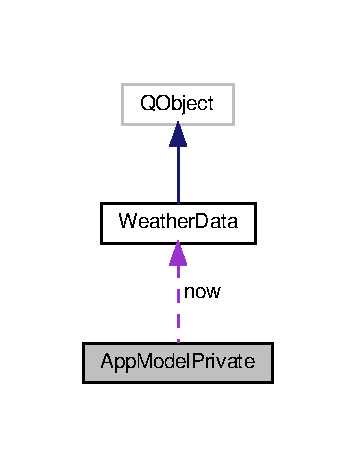
\includegraphics[width=171pt]{class_app_model_private__coll__graph}
\end{center}
\end{figure}
\subsection*{Public Member Functions}
\begin{DoxyCompactItemize}
\item 
\hyperlink{class_app_model_private_ac7e4e160306c7ff9c771d2dd34c243ac}{App\+Model\+Private} ()
\end{DoxyCompactItemize}
\subsection*{Public Attributes}
\begin{DoxyCompactItemize}
\item 
\hyperlink{class_weather_data}{Weather\+Data} \hyperlink{class_app_model_private_adacce6c96a2a7b0b825586a63a15bcac}{now}
\item 
bool \hyperlink{class_app_model_private_ab0434f387adadf9ed65183496fe80f77}{ready}
\item 
Q\+Timer \hyperlink{class_app_model_private_ad073c8bcf6739fd658009860e12aa72c}{request\+New\+Weather\+Timer}
\end{DoxyCompactItemize}


\subsection{Constructor \& Destructor Documentation}
\mbox{\Hypertarget{class_app_model_private_ac7e4e160306c7ff9c771d2dd34c243ac}\label{class_app_model_private_ac7e4e160306c7ff9c771d2dd34c243ac}} 
\index{App\+Model\+Private@{App\+Model\+Private}!App\+Model\+Private@{App\+Model\+Private}}
\index{App\+Model\+Private@{App\+Model\+Private}!App\+Model\+Private@{App\+Model\+Private}}
\subsubsection{\texorpdfstring{App\+Model\+Private()}{AppModelPrivate()}}
{\footnotesize\ttfamily App\+Model\+Private\+::\+App\+Model\+Private (\begin{DoxyParamCaption}{ }\end{DoxyParamCaption})\hspace{0.3cm}{\ttfamily [inline]}}



\subsection{Member Data Documentation}
\mbox{\Hypertarget{class_app_model_private_adacce6c96a2a7b0b825586a63a15bcac}\label{class_app_model_private_adacce6c96a2a7b0b825586a63a15bcac}} 
\index{App\+Model\+Private@{App\+Model\+Private}!now@{now}}
\index{now@{now}!App\+Model\+Private@{App\+Model\+Private}}
\subsubsection{\texorpdfstring{now}{now}}
{\footnotesize\ttfamily \hyperlink{class_weather_data}{Weather\+Data} App\+Model\+Private\+::now}

\mbox{\Hypertarget{class_app_model_private_ab0434f387adadf9ed65183496fe80f77}\label{class_app_model_private_ab0434f387adadf9ed65183496fe80f77}} 
\index{App\+Model\+Private@{App\+Model\+Private}!ready@{ready}}
\index{ready@{ready}!App\+Model\+Private@{App\+Model\+Private}}
\subsubsection{\texorpdfstring{ready}{ready}}
{\footnotesize\ttfamily bool App\+Model\+Private\+::ready}

\mbox{\Hypertarget{class_app_model_private_ad073c8bcf6739fd658009860e12aa72c}\label{class_app_model_private_ad073c8bcf6739fd658009860e12aa72c}} 
\index{App\+Model\+Private@{App\+Model\+Private}!request\+New\+Weather\+Timer@{request\+New\+Weather\+Timer}}
\index{request\+New\+Weather\+Timer@{request\+New\+Weather\+Timer}!App\+Model\+Private@{App\+Model\+Private}}
\subsubsection{\texorpdfstring{request\+New\+Weather\+Timer}{requestNewWeatherTimer}}
{\footnotesize\ttfamily Q\+Timer App\+Model\+Private\+::request\+New\+Weather\+Timer}



The documentation for this class was generated from the following file\+:\begin{DoxyCompactItemize}
\item 
\hyperlink{appmodel_8cpp}{appmodel.\+cpp}\end{DoxyCompactItemize}

\hypertarget{class_weather_data}{}\section{Weather\+Data Class Reference}
\label{class_weather_data}\index{Weather\+Data@{Weather\+Data}}


\mbox{[}0\mbox{]}  




{\ttfamily \#include $<$appmodel.\+h$>$}



Inheritance diagram for Weather\+Data\+:\nopagebreak
\begin{figure}[H]
\begin{center}
\leavevmode
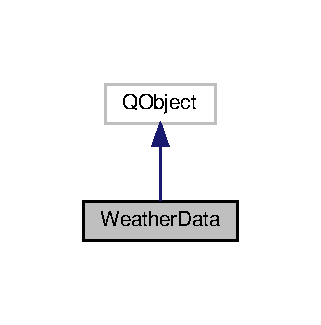
\includegraphics[width=154pt]{class_weather_data__inherit__graph}
\end{center}
\end{figure}
\subsection*{Signals}
\begin{DoxyCompactItemize}
\item 
void \hyperlink{class_weather_data_a23185106cf22ef8c57c96154e37b24d1}{data\+Changed} ()
\end{DoxyCompactItemize}
\subsection*{Public Member Functions}
\begin{DoxyCompactItemize}
\item 
\hyperlink{class_weather_data_aae42655299392d3f90feec9911a2dd60}{Weather\+Data} (Q\+Object $\ast$parent=0)
\item 
\hyperlink{class_weather_data_a48baeaa6b2a77d2a5e008159188416e8}{Weather\+Data} (const \hyperlink{class_weather_data}{Weather\+Data} \&other)
\item 
Q\+String \hyperlink{class_weather_data_a413b0ccf3fad036782ee5f5cb66f9a62}{day\+Of\+Week} () const
\item 
Q\+String \hyperlink{class_weather_data_a5baf2d9cc08741d7af4a07d61df95ee4}{weather\+Icon} () const
\item 
Q\+String \hyperlink{class_weather_data_a63a3528697c8681bd32d4d170ec91f76}{weather\+Description} () const
\item 
Q\+String \hyperlink{class_weather_data_a5a193e8410e3a146de59bab224cd88f0}{temperature} () const
\item 
Q\+String \hyperlink{class_weather_data_af726e713890bd6d310fe4a718dd69c77}{pressure} () const
\item 
Q\+String \hyperlink{class_weather_data_a0a83b2ee5398eaba062e3c6fe9264a3d}{humidity} () const
\item 
void \hyperlink{class_weather_data_ab47f3e7cde6cf4d93dfb1750ac014f00}{set\+Day\+Of\+Week} (const Q\+String \&value)
\item 
void \hyperlink{class_weather_data_a2a8093aaf20e1fb3c63c429a4ae0a977}{set\+Weather\+Icon} (const Q\+String \&value)
\item 
void \hyperlink{class_weather_data_a68686722f2e0bbf5cb28f0fdc96e280d}{set\+Weather\+Description} (const Q\+String \&value)
\item 
void \hyperlink{class_weather_data_afee514cbb8713059cf8d0602b33cadf5}{set\+Temperature} (const Q\+String \&value)
\item 
void \hyperlink{class_weather_data_ad5b453016656864e2bc3a09fc75919a0}{set\+Pressure} (const Q\+String \&\hyperlink{class_weather_data_af726e713890bd6d310fe4a718dd69c77}{pressure})
\item 
void \hyperlink{class_weather_data_aad895695b5f0651c58657973f2140509}{set\+Humidity} (const Q\+String \&\hyperlink{class_weather_data_a0a83b2ee5398eaba062e3c6fe9264a3d}{humidity})
\end{DoxyCompactItemize}
\subsection*{Properties}
\begin{DoxyCompactItemize}
\item 
Q\+String \hyperlink{class_weather_data_a483043396f44ae957716ebb005644d0d}{day\+Of\+Week}
\item 
Q\+String \hyperlink{class_weather_data_aca04e1877e2d5bc6da0f1e9910553741}{weather\+Icon}
\item 
Q\+String \hyperlink{class_weather_data_a8b470bc177e317a6a6a6b51758724a1a}{weather\+Description}
\item 
Q\+String \hyperlink{class_weather_data_a2ee510e51cb81a6a479cd0af5f291e2c}{temperature}
\end{DoxyCompactItemize}


\subsection{Detailed Description}
\mbox{[}0\mbox{]} 

\subsection{Constructor \& Destructor Documentation}
\mbox{\Hypertarget{class_weather_data_aae42655299392d3f90feec9911a2dd60}\label{class_weather_data_aae42655299392d3f90feec9911a2dd60}} 
\index{Weather\+Data@{Weather\+Data}!Weather\+Data@{Weather\+Data}}
\index{Weather\+Data@{Weather\+Data}!Weather\+Data@{Weather\+Data}}
\subsubsection{\texorpdfstring{Weather\+Data()}{WeatherData()}\hspace{0.1cm}{\footnotesize\ttfamily [1/2]}}
{\footnotesize\ttfamily Weather\+Data\+::\+Weather\+Data (\begin{DoxyParamCaption}\item[{Q\+Object $\ast$}]{parent = {\ttfamily 0} }\end{DoxyParamCaption})\hspace{0.3cm}{\ttfamily [explicit]}}

\mbox{\Hypertarget{class_weather_data_a48baeaa6b2a77d2a5e008159188416e8}\label{class_weather_data_a48baeaa6b2a77d2a5e008159188416e8}} 
\index{Weather\+Data@{Weather\+Data}!Weather\+Data@{Weather\+Data}}
\index{Weather\+Data@{Weather\+Data}!Weather\+Data@{Weather\+Data}}
\subsubsection{\texorpdfstring{Weather\+Data()}{WeatherData()}\hspace{0.1cm}{\footnotesize\ttfamily [2/2]}}
{\footnotesize\ttfamily Weather\+Data\+::\+Weather\+Data (\begin{DoxyParamCaption}\item[{const \hyperlink{class_weather_data}{Weather\+Data} \&}]{other }\end{DoxyParamCaption})}

Here is the call graph for this function\+:\nopagebreak
\begin{figure}[H]
\begin{center}
\leavevmode
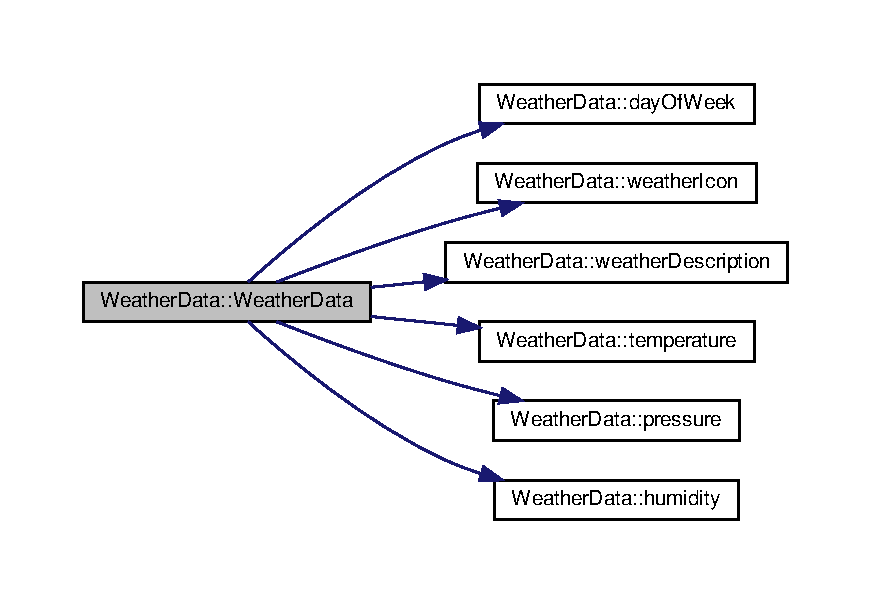
\includegraphics[width=350pt]{class_weather_data_a48baeaa6b2a77d2a5e008159188416e8_cgraph}
\end{center}
\end{figure}


\subsection{Member Function Documentation}
\mbox{\Hypertarget{class_weather_data_a23185106cf22ef8c57c96154e37b24d1}\label{class_weather_data_a23185106cf22ef8c57c96154e37b24d1}} 
\index{Weather\+Data@{Weather\+Data}!data\+Changed@{data\+Changed}}
\index{data\+Changed@{data\+Changed}!Weather\+Data@{Weather\+Data}}
\subsubsection{\texorpdfstring{data\+Changed}{dataChanged}}
{\footnotesize\ttfamily void Weather\+Data\+::data\+Changed (\begin{DoxyParamCaption}{ }\end{DoxyParamCaption})\hspace{0.3cm}{\ttfamily [signal]}}

Here is the caller graph for this function\+:\nopagebreak
\begin{figure}[H]
\begin{center}
\leavevmode
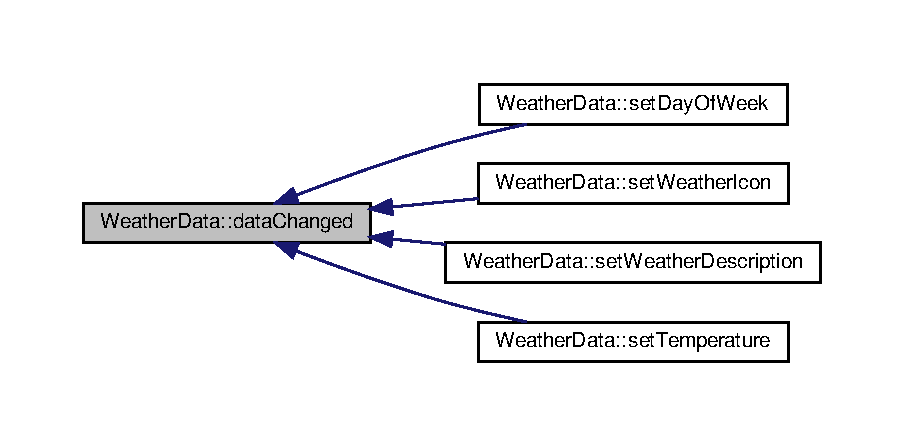
\includegraphics[width=350pt]{class_weather_data_a23185106cf22ef8c57c96154e37b24d1_icgraph}
\end{center}
\end{figure}
\mbox{\Hypertarget{class_weather_data_a413b0ccf3fad036782ee5f5cb66f9a62}\label{class_weather_data_a413b0ccf3fad036782ee5f5cb66f9a62}} 
\index{Weather\+Data@{Weather\+Data}!day\+Of\+Week@{day\+Of\+Week}}
\index{day\+Of\+Week@{day\+Of\+Week}!Weather\+Data@{Weather\+Data}}
\subsubsection{\texorpdfstring{day\+Of\+Week()}{dayOfWeek()}}
{\footnotesize\ttfamily Q\+String Weather\+Data\+::day\+Of\+Week (\begin{DoxyParamCaption}{ }\end{DoxyParamCaption}) const}

Here is the caller graph for this function\+:\nopagebreak
\begin{figure}[H]
\begin{center}
\leavevmode
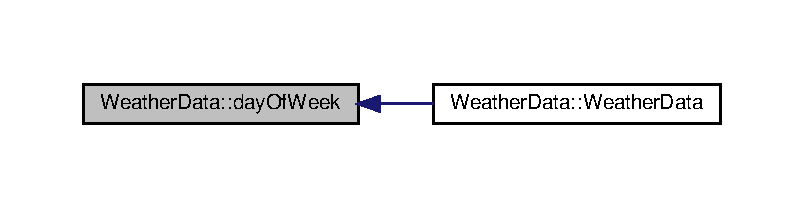
\includegraphics[width=350pt]{class_weather_data_a413b0ccf3fad036782ee5f5cb66f9a62_icgraph}
\end{center}
\end{figure}
\mbox{\Hypertarget{class_weather_data_a0a83b2ee5398eaba062e3c6fe9264a3d}\label{class_weather_data_a0a83b2ee5398eaba062e3c6fe9264a3d}} 
\index{Weather\+Data@{Weather\+Data}!humidity@{humidity}}
\index{humidity@{humidity}!Weather\+Data@{Weather\+Data}}
\subsubsection{\texorpdfstring{humidity()}{humidity()}}
{\footnotesize\ttfamily Q\+String Weather\+Data\+::humidity (\begin{DoxyParamCaption}{ }\end{DoxyParamCaption}) const}

Here is the caller graph for this function\+:\nopagebreak
\begin{figure}[H]
\begin{center}
\leavevmode
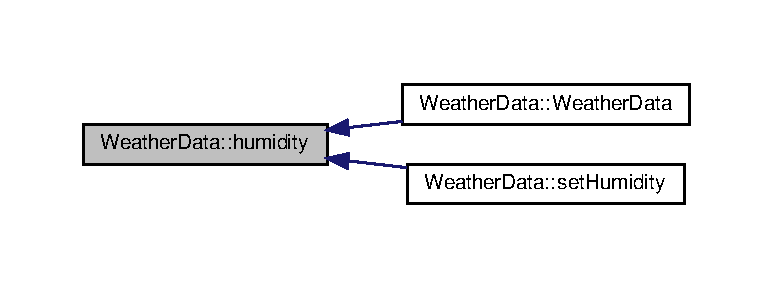
\includegraphics[width=350pt]{class_weather_data_a0a83b2ee5398eaba062e3c6fe9264a3d_icgraph}
\end{center}
\end{figure}
\mbox{\Hypertarget{class_weather_data_af726e713890bd6d310fe4a718dd69c77}\label{class_weather_data_af726e713890bd6d310fe4a718dd69c77}} 
\index{Weather\+Data@{Weather\+Data}!pressure@{pressure}}
\index{pressure@{pressure}!Weather\+Data@{Weather\+Data}}
\subsubsection{\texorpdfstring{pressure()}{pressure()}}
{\footnotesize\ttfamily Q\+String Weather\+Data\+::pressure (\begin{DoxyParamCaption}{ }\end{DoxyParamCaption}) const}

Here is the caller graph for this function\+:\nopagebreak
\begin{figure}[H]
\begin{center}
\leavevmode
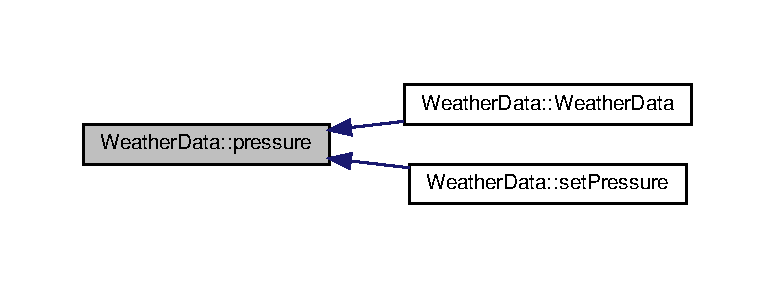
\includegraphics[width=350pt]{class_weather_data_af726e713890bd6d310fe4a718dd69c77_icgraph}
\end{center}
\end{figure}
\mbox{\Hypertarget{class_weather_data_ab47f3e7cde6cf4d93dfb1750ac014f00}\label{class_weather_data_ab47f3e7cde6cf4d93dfb1750ac014f00}} 
\index{Weather\+Data@{Weather\+Data}!set\+Day\+Of\+Week@{set\+Day\+Of\+Week}}
\index{set\+Day\+Of\+Week@{set\+Day\+Of\+Week}!Weather\+Data@{Weather\+Data}}
\subsubsection{\texorpdfstring{set\+Day\+Of\+Week()}{setDayOfWeek()}}
{\footnotesize\ttfamily void Weather\+Data\+::set\+Day\+Of\+Week (\begin{DoxyParamCaption}\item[{const Q\+String \&}]{value }\end{DoxyParamCaption})}

\mbox{\Hypertarget{class_weather_data_aad895695b5f0651c58657973f2140509}\label{class_weather_data_aad895695b5f0651c58657973f2140509}} 
\index{Weather\+Data@{Weather\+Data}!set\+Humidity@{set\+Humidity}}
\index{set\+Humidity@{set\+Humidity}!Weather\+Data@{Weather\+Data}}
\subsubsection{\texorpdfstring{set\+Humidity()}{setHumidity()}}
{\footnotesize\ttfamily void Weather\+Data\+::set\+Humidity (\begin{DoxyParamCaption}\item[{const Q\+String \&}]{humidity }\end{DoxyParamCaption})}

Here is the call graph for this function\+:\nopagebreak
\begin{figure}[H]
\begin{center}
\leavevmode
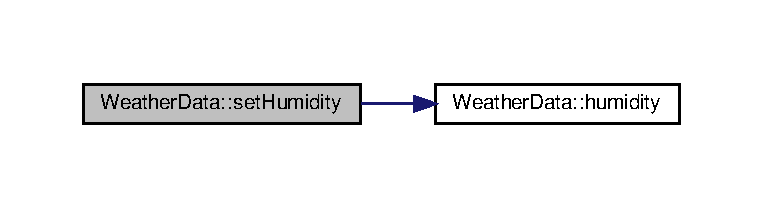
\includegraphics[width=350pt]{class_weather_data_aad895695b5f0651c58657973f2140509_cgraph}
\end{center}
\end{figure}
\mbox{\Hypertarget{class_weather_data_ad5b453016656864e2bc3a09fc75919a0}\label{class_weather_data_ad5b453016656864e2bc3a09fc75919a0}} 
\index{Weather\+Data@{Weather\+Data}!set\+Pressure@{set\+Pressure}}
\index{set\+Pressure@{set\+Pressure}!Weather\+Data@{Weather\+Data}}
\subsubsection{\texorpdfstring{set\+Pressure()}{setPressure()}}
{\footnotesize\ttfamily void Weather\+Data\+::set\+Pressure (\begin{DoxyParamCaption}\item[{const Q\+String \&}]{pressure }\end{DoxyParamCaption})}

Here is the call graph for this function\+:\nopagebreak
\begin{figure}[H]
\begin{center}
\leavevmode
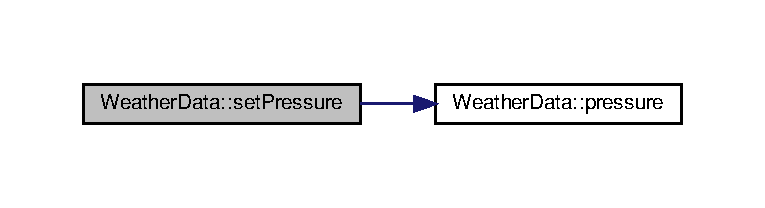
\includegraphics[width=350pt]{class_weather_data_ad5b453016656864e2bc3a09fc75919a0_cgraph}
\end{center}
\end{figure}
\mbox{\Hypertarget{class_weather_data_afee514cbb8713059cf8d0602b33cadf5}\label{class_weather_data_afee514cbb8713059cf8d0602b33cadf5}} 
\index{Weather\+Data@{Weather\+Data}!set\+Temperature@{set\+Temperature}}
\index{set\+Temperature@{set\+Temperature}!Weather\+Data@{Weather\+Data}}
\subsubsection{\texorpdfstring{set\+Temperature()}{setTemperature()}}
{\footnotesize\ttfamily void Weather\+Data\+::set\+Temperature (\begin{DoxyParamCaption}\item[{const Q\+String \&}]{value }\end{DoxyParamCaption})}

\mbox{\Hypertarget{class_weather_data_a68686722f2e0bbf5cb28f0fdc96e280d}\label{class_weather_data_a68686722f2e0bbf5cb28f0fdc96e280d}} 
\index{Weather\+Data@{Weather\+Data}!set\+Weather\+Description@{set\+Weather\+Description}}
\index{set\+Weather\+Description@{set\+Weather\+Description}!Weather\+Data@{Weather\+Data}}
\subsubsection{\texorpdfstring{set\+Weather\+Description()}{setWeatherDescription()}}
{\footnotesize\ttfamily void Weather\+Data\+::set\+Weather\+Description (\begin{DoxyParamCaption}\item[{const Q\+String \&}]{value }\end{DoxyParamCaption})}

\mbox{\Hypertarget{class_weather_data_a2a8093aaf20e1fb3c63c429a4ae0a977}\label{class_weather_data_a2a8093aaf20e1fb3c63c429a4ae0a977}} 
\index{Weather\+Data@{Weather\+Data}!set\+Weather\+Icon@{set\+Weather\+Icon}}
\index{set\+Weather\+Icon@{set\+Weather\+Icon}!Weather\+Data@{Weather\+Data}}
\subsubsection{\texorpdfstring{set\+Weather\+Icon()}{setWeatherIcon()}}
{\footnotesize\ttfamily void Weather\+Data\+::set\+Weather\+Icon (\begin{DoxyParamCaption}\item[{const Q\+String \&}]{value }\end{DoxyParamCaption})}

\mbox{\Hypertarget{class_weather_data_a5a193e8410e3a146de59bab224cd88f0}\label{class_weather_data_a5a193e8410e3a146de59bab224cd88f0}} 
\index{Weather\+Data@{Weather\+Data}!temperature@{temperature}}
\index{temperature@{temperature}!Weather\+Data@{Weather\+Data}}
\subsubsection{\texorpdfstring{temperature()}{temperature()}}
{\footnotesize\ttfamily Q\+String Weather\+Data\+::temperature (\begin{DoxyParamCaption}{ }\end{DoxyParamCaption}) const}

Here is the caller graph for this function\+:\nopagebreak
\begin{figure}[H]
\begin{center}
\leavevmode
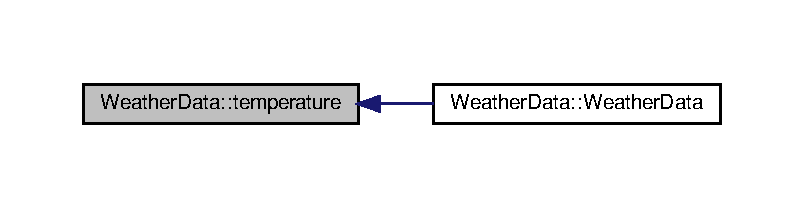
\includegraphics[width=350pt]{class_weather_data_a5a193e8410e3a146de59bab224cd88f0_icgraph}
\end{center}
\end{figure}
\mbox{\Hypertarget{class_weather_data_a63a3528697c8681bd32d4d170ec91f76}\label{class_weather_data_a63a3528697c8681bd32d4d170ec91f76}} 
\index{Weather\+Data@{Weather\+Data}!weather\+Description@{weather\+Description}}
\index{weather\+Description@{weather\+Description}!Weather\+Data@{Weather\+Data}}
\subsubsection{\texorpdfstring{weather\+Description()}{weatherDescription()}}
{\footnotesize\ttfamily Q\+String Weather\+Data\+::weather\+Description (\begin{DoxyParamCaption}{ }\end{DoxyParamCaption}) const}

Here is the caller graph for this function\+:\nopagebreak
\begin{figure}[H]
\begin{center}
\leavevmode
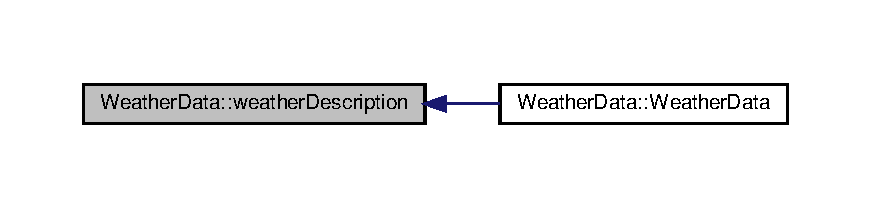
\includegraphics[width=350pt]{class_weather_data_a63a3528697c8681bd32d4d170ec91f76_icgraph}
\end{center}
\end{figure}
\mbox{\Hypertarget{class_weather_data_a5baf2d9cc08741d7af4a07d61df95ee4}\label{class_weather_data_a5baf2d9cc08741d7af4a07d61df95ee4}} 
\index{Weather\+Data@{Weather\+Data}!weather\+Icon@{weather\+Icon}}
\index{weather\+Icon@{weather\+Icon}!Weather\+Data@{Weather\+Data}}
\subsubsection{\texorpdfstring{weather\+Icon()}{weatherIcon()}}
{\footnotesize\ttfamily Q\+String Weather\+Data\+::weather\+Icon (\begin{DoxyParamCaption}{ }\end{DoxyParamCaption}) const}

Here is the caller graph for this function\+:\nopagebreak
\begin{figure}[H]
\begin{center}
\leavevmode
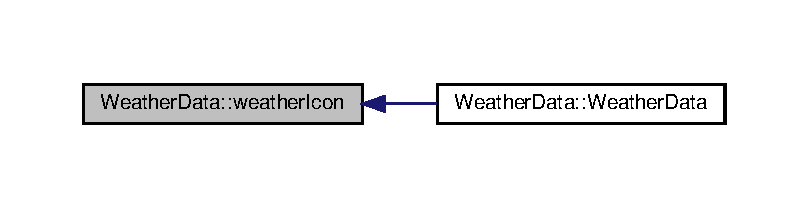
\includegraphics[width=350pt]{class_weather_data_a5baf2d9cc08741d7af4a07d61df95ee4_icgraph}
\end{center}
\end{figure}


\subsection{Property Documentation}
\mbox{\Hypertarget{class_weather_data_a483043396f44ae957716ebb005644d0d}\label{class_weather_data_a483043396f44ae957716ebb005644d0d}} 
\index{Weather\+Data@{Weather\+Data}!day\+Of\+Week@{day\+Of\+Week}}
\index{day\+Of\+Week@{day\+Of\+Week}!Weather\+Data@{Weather\+Data}}
\subsubsection{\texorpdfstring{day\+Of\+Week}{dayOfWeek}}
{\footnotesize\ttfamily Q\+String Weather\+Data\+::day\+Of\+Week\hspace{0.3cm}{\ttfamily [read]}, {\ttfamily [write]}}

\mbox{\Hypertarget{class_weather_data_a2ee510e51cb81a6a479cd0af5f291e2c}\label{class_weather_data_a2ee510e51cb81a6a479cd0af5f291e2c}} 
\index{Weather\+Data@{Weather\+Data}!temperature@{temperature}}
\index{temperature@{temperature}!Weather\+Data@{Weather\+Data}}
\subsubsection{\texorpdfstring{temperature}{temperature}}
{\footnotesize\ttfamily Q\+String Weather\+Data\+::temperature\hspace{0.3cm}{\ttfamily [read]}, {\ttfamily [write]}}

\mbox{\Hypertarget{class_weather_data_a8b470bc177e317a6a6a6b51758724a1a}\label{class_weather_data_a8b470bc177e317a6a6a6b51758724a1a}} 
\index{Weather\+Data@{Weather\+Data}!weather\+Description@{weather\+Description}}
\index{weather\+Description@{weather\+Description}!Weather\+Data@{Weather\+Data}}
\subsubsection{\texorpdfstring{weather\+Description}{weatherDescription}}
{\footnotesize\ttfamily Q\+String Weather\+Data\+::weather\+Description\hspace{0.3cm}{\ttfamily [read]}, {\ttfamily [write]}}

\mbox{\Hypertarget{class_weather_data_aca04e1877e2d5bc6da0f1e9910553741}\label{class_weather_data_aca04e1877e2d5bc6da0f1e9910553741}} 
\index{Weather\+Data@{Weather\+Data}!weather\+Icon@{weather\+Icon}}
\index{weather\+Icon@{weather\+Icon}!Weather\+Data@{Weather\+Data}}
\subsubsection{\texorpdfstring{weather\+Icon}{weatherIcon}}
{\footnotesize\ttfamily Q\+String Weather\+Data\+::weather\+Icon\hspace{0.3cm}{\ttfamily [read]}, {\ttfamily [write]}}

The icon value is based on Open\+Weather\+Map.\+org icon set. For details see \href{http://bugs.openweathermap.org/projects/api/wiki/Weather_Condition_Codes}{\tt http\+://bugs.\+openweathermap.\+org/projects/api/wiki/\+Weather\+\_\+\+Condition\+\_\+\+Codes}

e.\+g. 01d -\/$>$sunny day

The icon string will be translated to \href{http://openweathermap.org/img/w/01d.png}{\tt http\+://openweathermap.\+org/img/w/01d.\+png} 

The documentation for this class was generated from the following files\+:\begin{DoxyCompactItemize}
\item 
/home/jerome/projects/\+Weather\+Checking\+Rpi/weathercheckingrpi/\hyperlink{appmodel_8h}{appmodel.\+h}\item 
/home/jerome/projects/\+Weather\+Checking\+Rpi/weathercheckingrpi/\hyperlink{appmodel_8cpp}{appmodel.\+cpp}\end{DoxyCompactItemize}

\chapter{File Documentation}
\hypertarget{appmodel_8cpp}{}\section{appmodel.\+cpp File Reference}
\label{appmodel_8cpp}\index{appmodel.\+cpp@{appmodel.\+cpp}}
{\ttfamily \#include \char`\"{}appmodel.\+h\char`\"{}}\newline
{\ttfamily \#include $<$Q\+Json\+Document$>$}\newline
{\ttfamily \#include $<$Q\+Json\+Object$>$}\newline
{\ttfamily \#include $<$Q\+Json\+Array$>$}\newline
{\ttfamily \#include $<$Q\+String\+List$>$}\newline
{\ttfamily \#include $<$Q\+Timer$>$}\newline
{\ttfamily \#include $<$Q\+File$>$}\newline
{\ttfamily \#include $<$Q\+Url\+Query$>$}\newline
{\ttfamily \#include $<$Q\+Elapsed\+Timer$>$}\newline
{\ttfamily \#include $<$Q\+Logging\+Category$>$}\newline
{\ttfamily \#include $<$Q\+Dir$>$}\newline
{\ttfamily \#include $<$Q\+Core\+Application$>$}\newline
{\ttfamily \#include \char`\"{}zambretti/\+Zambretti.\+h\char`\"{}}\newline
{\ttfamily \#include \char`\"{}sensor/\+Metrics\+Average.\+h\char`\"{}}\newline
{\ttfamily \#include \char`\"{}sensor/sensor.\+h\char`\"{}}\newline
{\ttfamily \#include $<$iostream$>$}\newline
Include dependency graph for appmodel.\+cpp\+:
\nopagebreak
\begin{figure}[H]
\begin{center}
\leavevmode
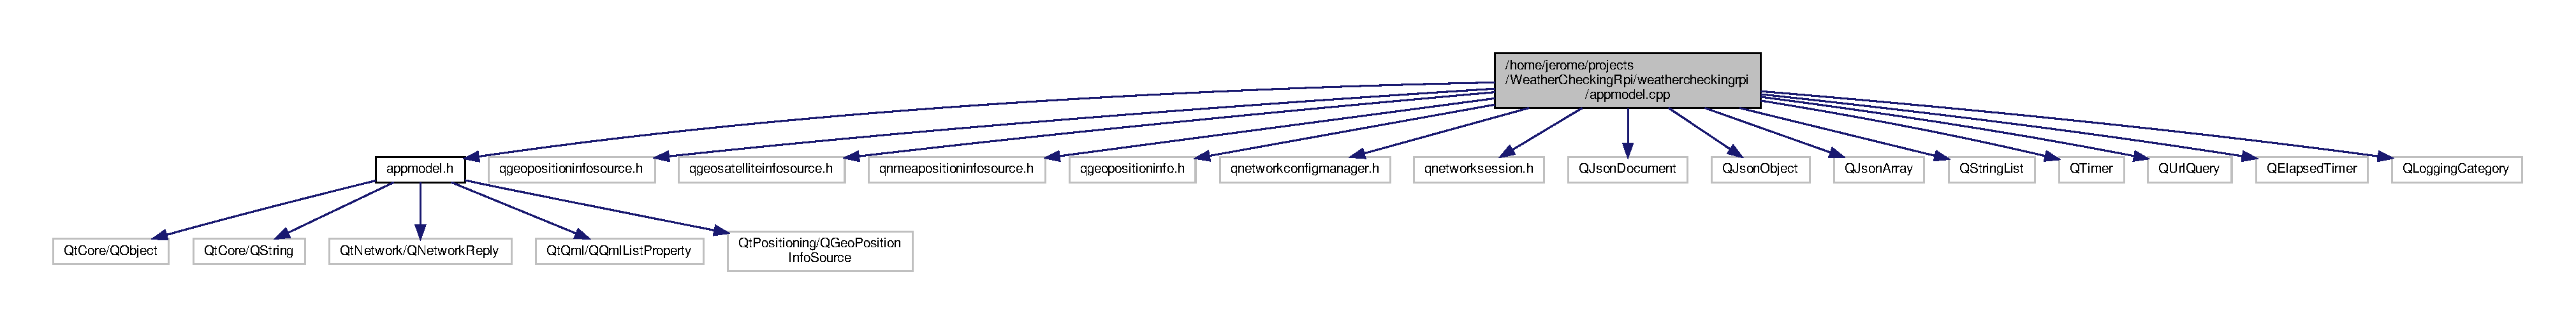
\includegraphics[width=350pt]{appmodel_8cpp__incl}
\end{center}
\end{figure}
\subsection*{Classes}
\begin{DoxyCompactItemize}
\item 
class \hyperlink{class_app_model_private}{App\+Model\+Private}
\end{DoxyCompactItemize}
\subsection*{Macros}
\begin{DoxyCompactItemize}
\item 
\#define \hyperlink{appmodel_8cpp_a6845ca0b7bf6295d883ba9ad80c2338c}{Z\+E\+R\+O\+\_\+\+K\+E\+L\+V\+IN}~273.\+15
\end{DoxyCompactItemize}


\subsection{Macro Definition Documentation}
\mbox{\Hypertarget{appmodel_8cpp_a6845ca0b7bf6295d883ba9ad80c2338c}\label{appmodel_8cpp_a6845ca0b7bf6295d883ba9ad80c2338c}} 
\index{appmodel.\+cpp@{appmodel.\+cpp}!Z\+E\+R\+O\+\_\+\+K\+E\+L\+V\+IN@{Z\+E\+R\+O\+\_\+\+K\+E\+L\+V\+IN}}
\index{Z\+E\+R\+O\+\_\+\+K\+E\+L\+V\+IN@{Z\+E\+R\+O\+\_\+\+K\+E\+L\+V\+IN}!appmodel.\+cpp@{appmodel.\+cpp}}
\subsubsection{\texorpdfstring{Z\+E\+R\+O\+\_\+\+K\+E\+L\+V\+IN}{ZERO\_KELVIN}}
{\footnotesize\ttfamily \#define Z\+E\+R\+O\+\_\+\+K\+E\+L\+V\+IN~273.\+15}


\hypertarget{appmodel_8h}{}\section{appmodel.\+h File Reference}
\label{appmodel_8h}\index{appmodel.\+h@{appmodel.\+h}}
{\ttfamily \#include $<$Qt\+Core/\+Q\+Object$>$}\newline
{\ttfamily \#include $<$Qt\+Core/\+Q\+String$>$}\newline
{\ttfamily \#include $<$Q\+Json\+Document$>$}\newline
{\ttfamily \#include \char`\"{}sensor/\+Metrics\+Average.\+h\char`\"{}}\newline
{\ttfamily \#include \char`\"{}sensor/sensor.\+h\char`\"{}}\newline
{\ttfamily \#include \char`\"{}zambretti/\+Zambretti.\+h\char`\"{}}\newline
Include dependency graph for appmodel.\+h\+:
\nopagebreak
\begin{figure}[H]
\begin{center}
\leavevmode
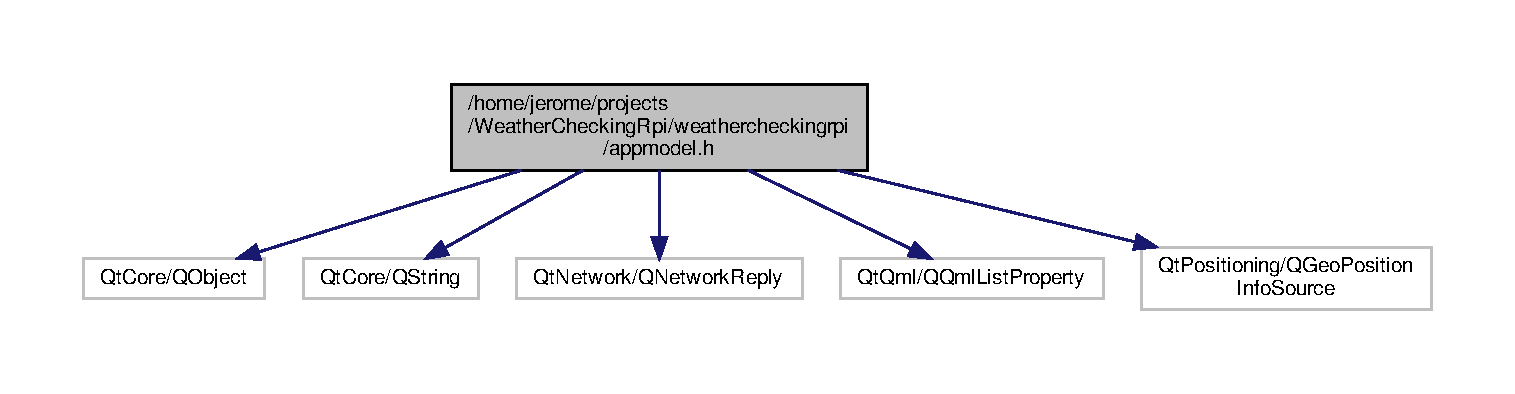
\includegraphics[width=350pt]{appmodel_8h__incl}
\end{center}
\end{figure}
This graph shows which files directly or indirectly include this file\+:
\nopagebreak
\begin{figure}[H]
\begin{center}
\leavevmode
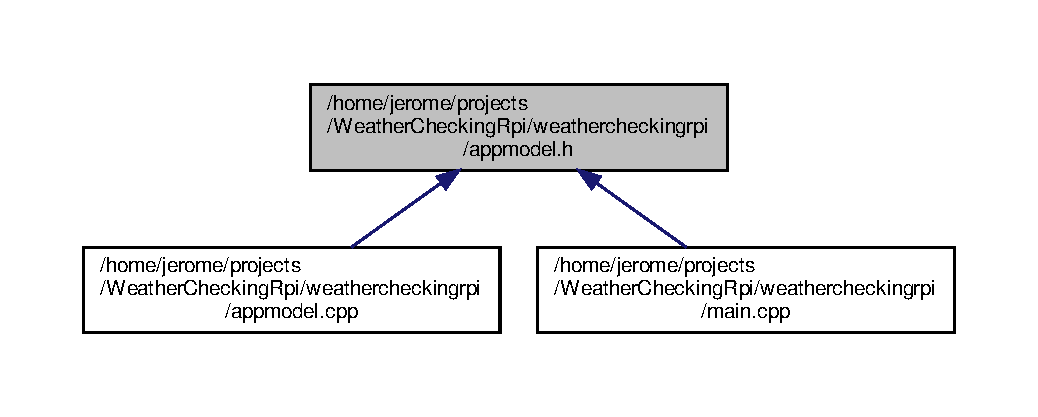
\includegraphics[width=232pt]{appmodel_8h__dep__incl}
\end{center}
\end{figure}
\subsection*{Classes}
\begin{DoxyCompactItemize}
\item 
class \hyperlink{class_weather_data}{Weather\+Data}
\item 
class \hyperlink{class_app_model}{App\+Model}
\end{DoxyCompactItemize}

\hypertarget{main_8cpp}{}\section{/home/jerome/projects/\+Weather\+Checking\+Rpi/weathercheckingrpi/main.cpp File Reference}
\label{main_8cpp}\index{/home/jerome/projects/\+Weather\+Checking\+Rpi/weathercheckingrpi/main.\+cpp@{/home/jerome/projects/\+Weather\+Checking\+Rpi/weathercheckingrpi/main.\+cpp}}
{\ttfamily \#include $<$Qt\+Gui/\+Q\+Gui\+Application$>$}\newline
{\ttfamily \#include $<$Qt\+Quick/\+Q\+Quick\+View$>$}\newline
{\ttfamily \#include $<$Qt\+Qml/\+Q\+Qml\+Engine$>$}\newline
{\ttfamily \#include $<$Qt\+Qml/\+Q\+Qml\+Context$>$}\newline
{\ttfamily \#include $<$Qt\+Quick/\+Q\+Quick\+Item$>$}\newline
{\ttfamily \#include $<$Q\+Logging\+Category$>$}\newline
{\ttfamily \#include \char`\"{}appmodel.\+h\char`\"{}}\newline
Include dependency graph for main.\+cpp\+:\nopagebreak
\begin{figure}[H]
\begin{center}
\leavevmode
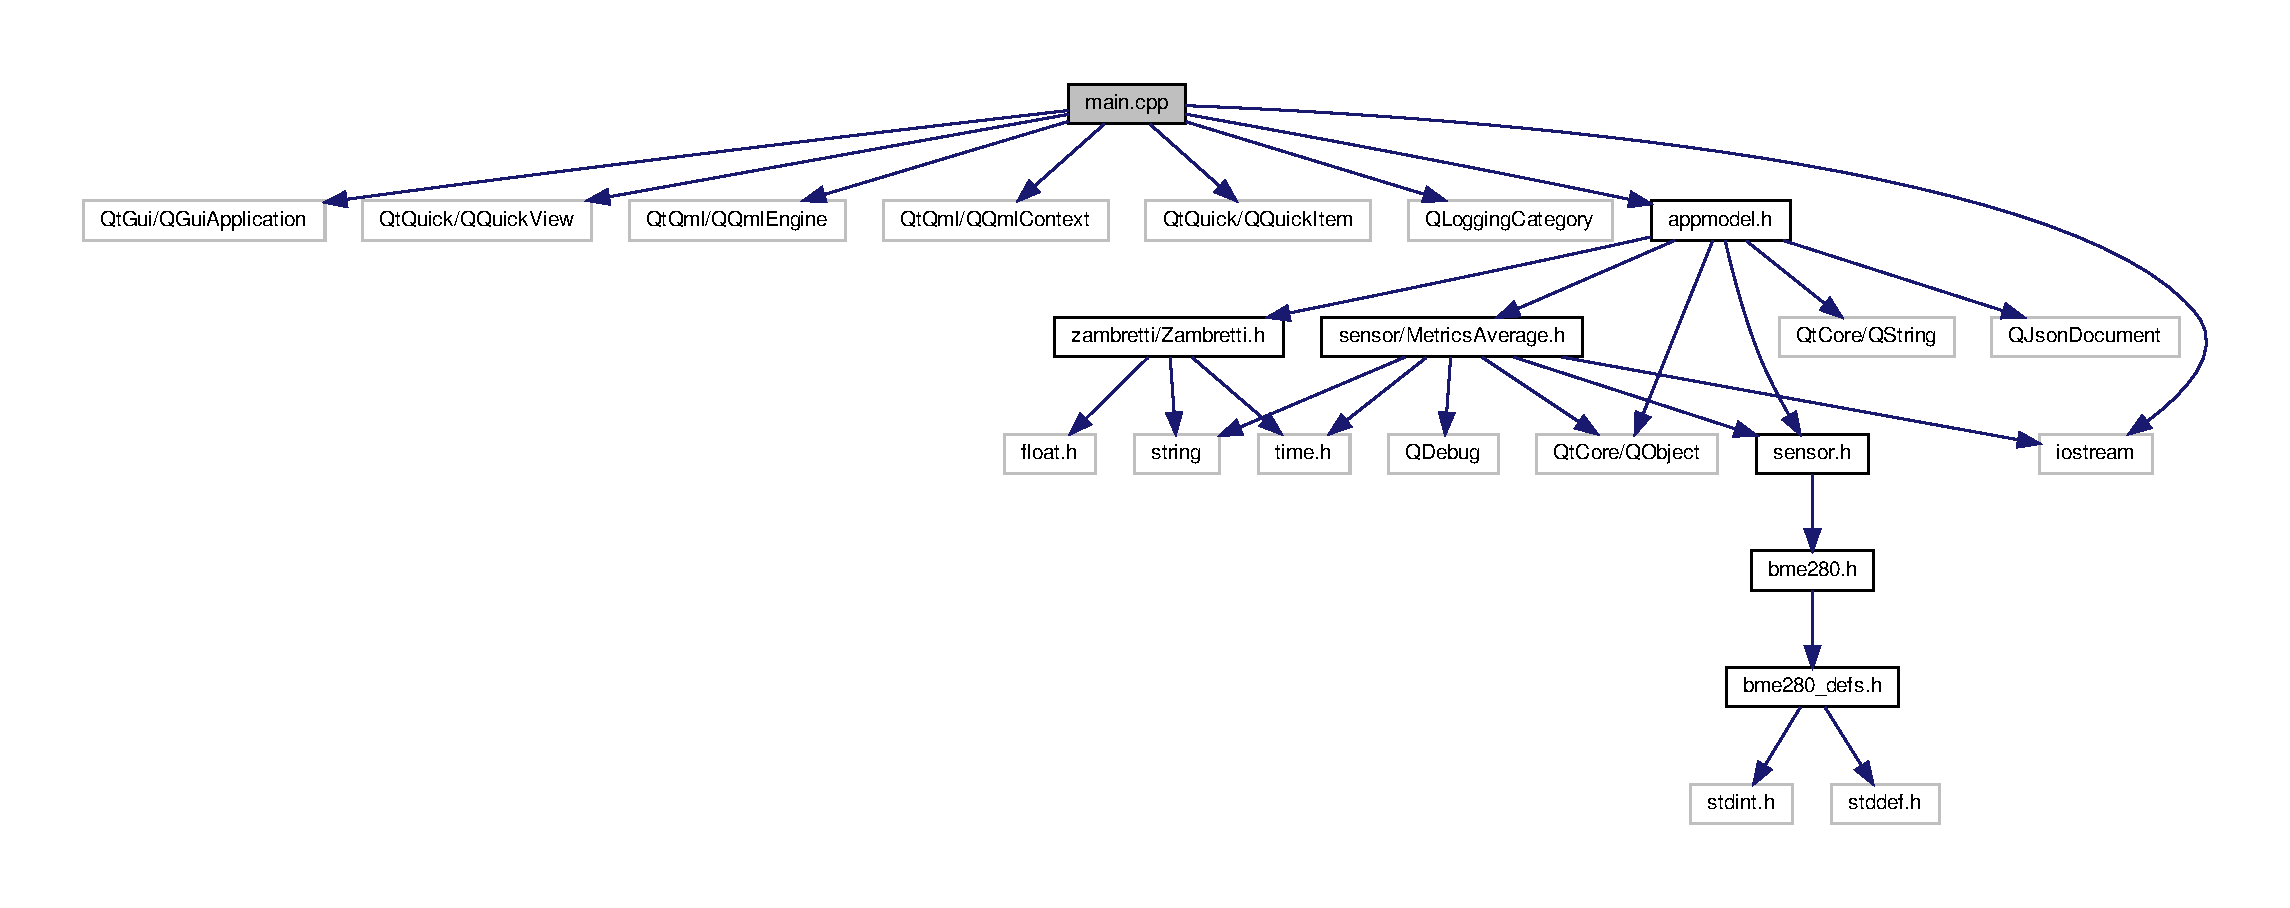
\includegraphics[width=350pt]{main_8cpp__incl}
\end{center}
\end{figure}
\subsection*{Functions}
\begin{DoxyCompactItemize}
\item 
int \hyperlink{main_8cpp_a0ddf1224851353fc92bfbff6f499fa97}{main} (int argc, char $\ast$argv\mbox{[}$\,$\mbox{]})
\begin{DoxyCompactList}\small\item\em \mbox{[}0\mbox{]} \end{DoxyCompactList}\end{DoxyCompactItemize}


\subsection{Function Documentation}
\mbox{\Hypertarget{main_8cpp_a0ddf1224851353fc92bfbff6f499fa97}\label{main_8cpp_a0ddf1224851353fc92bfbff6f499fa97}} 
\index{main.\+cpp@{main.\+cpp}!main@{main}}
\index{main@{main}!main.\+cpp@{main.\+cpp}}
\subsubsection{\texorpdfstring{main()}{main()}}
{\footnotesize\ttfamily int main (\begin{DoxyParamCaption}\item[{int}]{argc,  }\item[{char $\ast$}]{argv\mbox{[}$\,$\mbox{]} }\end{DoxyParamCaption})}



\mbox{[}0\mbox{]} 

\mbox{[}0\mbox{]}

\mbox{[}1\mbox{]} 
%--- End generated contents ---

% Index
\backmatter
\newpage
\phantomsection
\clearemptydoublepage
\addcontentsline{toc}{chapter}{Index}
\printindex

\end{document}
